\section{Result 2: Flips Alone Do Not Diagnose a Need for More Bits} % nocheck: section number
\label{sec:sameprec}
\label{sec:refs}

\begin{figure*}[t]
\centering
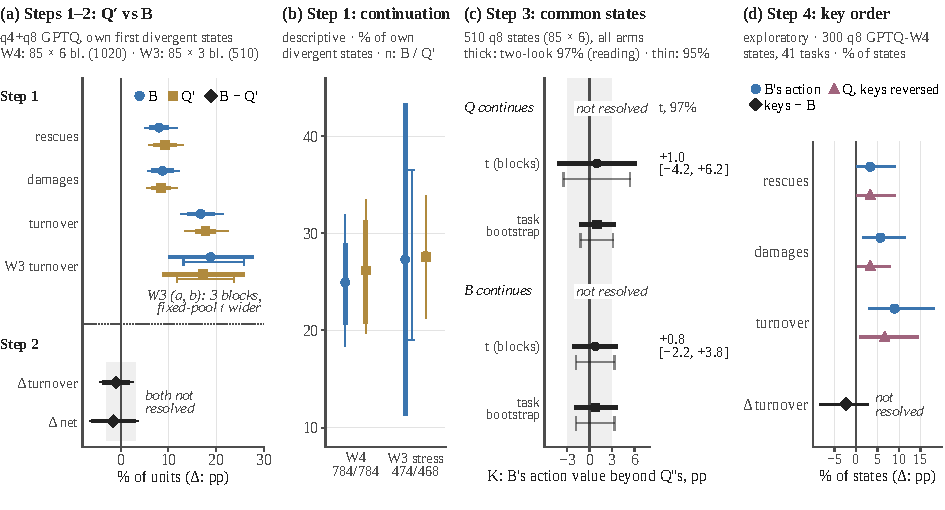
\includegraphics[width=\textwidth]{figures/f11_refs_quad.pdf}
\caption{Reference interventions, each in its own population (subtitles); comparisons are paired only within a panel, nothing is subtracted across panels, and references are not subtracted from B's turnover. Baseline: Q's action, same continuation. (a,b)~Q$'$ frozen before outcomes; shaded: $\pm$3\pp{} behind the paired differences. (c)~Pre-registered at three blocks; six-block extension and two-look rule fixed after the unresolved first look, before any extension output; a reading needs both the $t$ and task-cluster bootstrap intervals. (d)~Exploratory, code frozen before outcomes; bar: wider of block and crossed bootstrap 95\%. Thick / thin: (a,b) fixed-pool / new-task 95\% (thin beside thick when nested; with three W3 blocks the fixed-pool $t$ is wider); (c) as in its subtitle. Values: Table~\ref{tab:refsfull}.} % src: analysis/fork/out/sameprec_20261004T070601Z.json; analysis/fork/out/sameprec_20261004T070601Z.md; analysis/fork/out/sameprec_w3_20261004T070607Z.json; analysis/fork/out/sameprec_w3_20261004T070607Z.md; docs/insights/SAMEPREC_PROTOCOL.md; analysis/fork/out/commonstate_q8ext_20261003T231159Z.json; analysis/fork/out/commonstate_q8ext_20261003T231159Z.md; docs/insights/COMMONSTATE_SOURCES_PROTOCOL.md; analysis/fork/out/keyorder_20261005T204349Z.json; analysis/fork/out/keyorder_20261005T204349Z.md; analysis/fork/keyorder/eligibility_v1.md; docs/insights/KEYORDER_PERTURB_PROTOCOL.md; paper/latex/figures/provenance.json (f11_refs_quad; panels a-b: sameprec, sameprec_w3, incl. pooled.paired.dG and n_states; c: commonstate_q8ext, t97 labels as in appendix_refs_full.tex; d: keyorder); analysis/fork/out/sameprec_split_20261002T145148Z.md
\label{fig:refs}
\end{figure*}

\paragraph{The question and its three designs.} If the consequences in \S\ref{sec:value} required a higher bit width, a same-bit-width substitution should produce markedly fewer of them. Three reference designs test this in four steps (Figure~\ref{fig:refs}; all values in Table~\ref{tab:refsfull}). Each is compared with B's action only within its own population and never subtracted from B's turnover to obtain a precision-specific effect. % nocheck: step labels

\paragraph{Step 1: a higher bit width is not necessary for two-sided flips or continuation dependence.} At W4 (six blocks, the longest complete prefix under the frozen rule), Q$'$'s action both rescues and damages units, each with a fixed-pool 95\% lower bound above zero (Figure~\ref{fig:refs}a), and its effect is continuation dependent at some of its divergent states, as B's is (Figure~\ref{fig:refs}b). % src: docs/insights/SAMEPREC_PROTOCOL.md (A1.3, 95% lower bound); analysis/fork/out/sameprec_20261004T070601Z.md (TL;DR; Full pool; On divergent states; analysis set K = 6); analysis/fork/out/sameprec_20261004T070601Z.json (pooled.same.rescue/damage.crossed_ci95)
A W3 stress pair shows the same when only the W3 checkpoint is swapped (Figure~\ref{fig:refs}a, Appendix~\ref{app:qprime}). We do not claim the turnovers are equal: neither pair is equivalent within $\pm$3\pp{}. % src: analysis/fork/out/sameprec_w3_20261004T070607Z.md (TL;DR; Full pool, pool rows); analysis/fork/out/sameprec_20261004T070601Z.md (Amendment A1 table)

\paragraph{Step 2: because each design picks its own divergent states, this comparison cannot measure what B adds.} Flips found by only one design cannot be read as caused by precision, nor flips found by both as not caused by it. The action-side net difference, $-1.6$\pp{} (B minus Q$'$; fixed pool [$-6.2$, $+3.0$], new tasks [$-6.5$, $+3.6$]), is not resolved (Figure~\ref{fig:refs}a, $\Delta$ net) and compares two selection-and-replacement protocols, not two actions at one state (Appendix~\ref{app:qprime}). % src: analysis/fork/out/sameprec_split_20261002T145148Z.md (TL;DR; §3); analysis/fork/out/sameprec_20261004T070601Z.json (pooled.paired.dG.crossed_ci95); analysis/fork/out/sameprec_20261004T070601Z.md (Paired differences, pool row)

\paragraph{Step 3: at common states, B's extra action value over Q$'$ is not resolved, and equivalence is not shown.} At 510 ordinary q8 GPTQ-W4 states (85 tasks $\times$ 6 blocks) shared by all arms, B's action adds $K=+1.0$\pp{} beyond Q$'$'s under Q's continuation (two-look 97\% $t$ [$-4.2$, $+6.2$]) and $+0.8$\pp{} under B's ([$-2.2$, $+3.8$]; Figure~\ref{fig:refs}c). The design was pre-registered at three blocks and its first look was unresolved; dated amendments then fixed a six-block extension and a two-look reading, before any extension run had produced output. Without the 26 of the 510 states at which earlier studies had already produced outcomes, the two-look reading is unchanged. Neither value is resolved under the protocol-designated two-look reading, and equivalence is not shown (all intervals in Appendix~\ref{app:commonstate}). % src: docs/insights/COMMONSTATE_SOURCES_PROTOCOL.md (§2, §5, §6; A1.1, A1.3; D2.1; D2.2; D2.7); analysis/fork/out/commonstate_q8ext_20261003T231159Z.md (TL;DR; Key estimand table, t95 and t90; Two-look reading table, t97 and t94; Sensitivity without the D2.1 states); analysis/fork/out/commonstate_q4_20261004T001159Z.md (TL;DR, q4 K)

\paragraph{Step 4: an outcome can change while the tool operation stays identical.} At 300 q8 GPTQ-W4 first divergent states where Q's action is one tool call with at least two argument keys (41 tasks; airline 187, retail 113), we reverse the top-level key order; the call was checked to parse and execute identically, so only the tokens the agent reads change. This changes outcomes, as B's action on the same states does (Figure~\ref{fig:refs}d); the difference in turnover, $-2.3$\pp{} [$-8.4$, $+2.9$], is not resolved, and we claim no equivalence. Some outcome changes therefore arise without any change to the tool operation. This covers only these states and this one change, not free-text or other representation changes, and is not a perturbation curve (Appendix~\ref{app:keyorder}). % src: analysis/fork/out/keyorder_20261005T204349Z.md; analysis/fork/keyorder/eligibility_v1.md; docs/insights/KEYORDER_PERTURB_PROTOCOL.md (intervals: widest of block and crossed bootstrap on the pooled ratio)

The presence of flips alone therefore does not show that a decision needs B: sensitivity to an action, the value higher precision adds at a state, and the gain of a given upgrade need separate measurements.


% Scope matrix (replaces the former scope table): declared early so it can occupy a bottom float on a main-text page.
% R2 review: stronger tints plus a glyph per state (reads in greyscale); appendix pointers get their own style; the
% same-precision reference column is folded into "What it extends"; BFCL and RTN-W3 cells split into two coloured sub-rows.
% Cell key: \cSeen (palB!15, bullet; neutral, R3 review: green only for an interval excluding zero, positive) two-sided consequences seen; \cPos (palRescue!48, up-triangle) / \cNeg (palDamage!36, down-triangle) interval excludes zero, positive / negative; \cNR (gray!30, open circle) not resolved; white "--" not available; italic grey "App." reported in the appendix only.
\begin{table*}[!b]
% src: analysis/fork/out/ghf_20261001T211519Z.md (q8 RTN-W3, divergent-state H/F; crossed F); analysis/fork/out/dev_all_20261001T070326Z.md (q8:rtn_w3 row: G -0.4 [-3.8, +3.0]); analysis/fork/out/ext_20261001T135106Z.md (TL;DR; W4:bfcl pooled); analysis/fork/out/newmethod_m24_20261004T024453Z.md; analysis/fork/out/newmethod_m24_20261004T024453Z.json (tau2.cells.*.all_states_pp); docs/insights/NEWMETHOD_PANEL_PROTOCOL.md (A3); analysis/fork/out/newmethod_q8_20261004T051538Z.md; analysis/fork/out/newmethod_q8_20261004T051538Z.json (tau2.contrasts; fidelity.cells.*.KLu_mean); analysis/fork/out/sameprec_w3_20261004T070607Z.md (TL;DR)
\centering\footnotesize\setlength{\tabcolsep}{4pt}\renewcommand{\arraystretch}{1.08}
\setlength{\aboverulesep}{0pt}\setlength{\belowrulesep}{0pt}\setlength{\fboxsep}{1.5pt} % nocheck: colour/layout
\newcommand{\cSeen}{\cellcolor{palB!15}$\bullet$\,}\newcommand{\cPos}{\cellcolor{palRescue!48}$\blacktriangle$\,}\newcommand{\cNeg}{\cellcolor{palDamage!36}$\blacktriangledown$\,}\newcommand{\cNR}{\cellcolor{gray!30}$\circ$\,}\newcommand{\cApp}[1]{\textcolor{black!55}{\itshape #1}}\newcommand{\swatch}[2]{\fcolorbox{black!35}{#1}{\makebox[0.9em]{\scriptsize #2}}} % nocheck: colour/layout
\newcommand{\sep}{\arrayrulecolor{black!15}\midrule[0.3pt]\arrayrulecolor{black}} % nocheck: colour/layout
\begin{tabular}{@{}P{5.0cm}P{2.6cm}P{4.6cm}P{2.95cm}@{}}
\toprule
\textbf{Scope check} (population) & \textbf{Two-sided seen?} & \textbf{Net / gain resolved?} & \textbf{What it extends} \\
\midrule
\textbf{BFCL multi-turn} (q4/q8 W4, no simulated user) & \cSeen turnover 5.2--15.2\% & \cNR pool net $+0.1$ [$-1.0$, $+1.2$], not resolved & two-sided; no pooled gain \\
 & \cellcolor{palB!15} & \cNeg q4 AWQ-style net $-3.8$ [$-6.5$, $-1.3$] & \\
\sep
\textbf{ALFWorld} (q8 W4, 134 games, no simulated user) & \cSeen turnover 21.6--24.6\% & \cNR pool net $-3.7$ [$-9.7$, $+1.9$], not resolved & two-sided; no pooled gain \\
\sep
\textbf{Mistral-Small-3.2-24B} (GPTQ/RTN-W4, ordinary BF16-sourced states, 83 tasks) & \cSeen GPTQ rescues 4.6, damages 5.4\pp{} & \cNR no mode's net resolved & second family; no first-divergence or Q$'$ data \\
\sep
\textbf{Lower-bit stress} (q8 RTN-W3, one of five stress configurations; exploratory; 255 first divergences, 3 blocks) & \cApp{reported in App.~\ref{app:tables}} & \cNR net $\Gall$ $-0.4$ [$-3.8$, $+3.0$], new tasks [$-4.7$, $+3.9$], not resolved & $H$, $F$ gains when degraded; not W4 \\
 & & \cPos gain on divergent states: takeover $H=+15.3$, joint $F=+18.4$ [9.4, 28.2]\pp{} & \cApp{Q$'$ ref.: GPTQ-W3 only (\S\ref{sec:sameprec}), not RTN-W3} \\
\sep
\textbf{QuaRot / SpinQuant} (q8 W4A4, ordinary BF16-sourced states, 3 blocks) & \cApp{reported in App.~\ref{app:scope}} & \cNR value contrast $+1.2$ [$-4.7$, $+7.1$], not resolved & KL 0.165 vs 0.199: lower KL, no value order \\
\sep
\textbf{KV-cache precision} (KV8: q4/q8 first divergences; KIVI-2/4: q8 ordinary states) & \cSeen KV8 turnover 6.5--8.1\% & \cNR KIVI-2/4 vs KV8 not resolved & two-sided at KV8; no KIVI order \\
\bottomrule
\end{tabular}
\caption{Scope matrix, with populations kept separate (Appendix~\ref{app:scope}). Cells: \swatch{palB!15}{$\bullet$}~two-sided consequences seen; \swatch{palRescue!48}{$\blacktriangle$}~/~\swatch{palDamage!36}{$\blacktriangledown$}~interval excludes zero (positive / negative); \swatch{gray!30}{$\circ$}~not resolved; \cApp{italic grey}: reported in the appendix only. No scope check has a same-precision (Q$'$) reference; the only one outside the W4 pair is the GPTQ-W3 pair (\S\ref{sec:sameprec}). BFCL and ALFWorld use one run per item, with post hoc item-bootstrap 95\% intervals; the QuaRot/SpinQuant and RTN-W3 $F$ intervals are crossed 95\%, the RTN-W3 net gives fixed-pool and new-task 95\%.}
\label{tab:scope}
\end{table*}
